The probe was successfully run on the list of URIs generated by the homepage-only crawler described in \autoref{homepages-crawler}.
A histogram of the differences between the \texttt{tcptraceroute} result for the serving domain and the minimum TTL value required to obtain each file is show in Figure \ref{fig_gcprobehist}.
This histogram appears to show a bifurcation between files that were received within 4 hops of the estimated distance to the hosting domain, and files which were received more than 8 hops earlier than the estimated distance.
\begin{figure}
	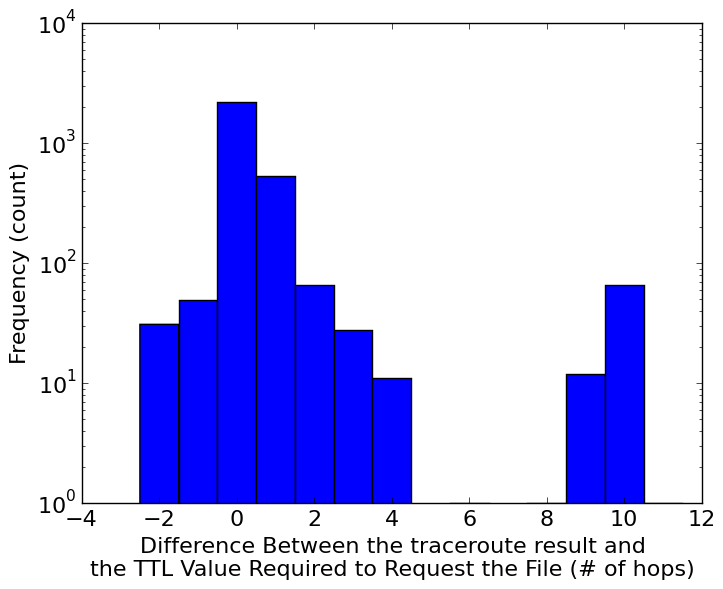
\includegraphics[width=\columnwidth]{figures/gcprobehist}
	\caption{
		A histogram showing how often a file request succeeded with a TTL value less than the number of hops to the server (as estimated by \texttt{tcptraceroute}~\cite{Toren2006}).
		A zero value on the x-axis represents files which were not received until the TTL value of the request was set to the result of the \texttt{tcptraceroute}.
		Larger values on the x-axis represent files which were received when the TTL value of the request was less than the result of the \texttt{tcptraceroute}.
		Negative values represent files which were not received until the TTL value of the request was set to be greater than the result of the \texttt{tcptraceroute}.
		Files which were not received even when the request was sent with a TTL value 3 greater than the \texttt{tcptraceroute} result are not shown.
	}
	\label{fig_gcprobehist}
\end{figure}

However, further analysis shows that the estimated distance to all 11 of the hosting domains for all of the files in the latter group is 30, the maximum number of hops that \texttt{tcptraceroute} analyzes before giving up.
Indeed, for several of these domains, the output from a first \texttt{tcptraceroute} shows that there is no response from any nodes past the first few.
However, for 10 of the 11 domains in question, repeated \texttt{tcptraceroutes} eventually place the estimated distances between 18 and 22 hops away.
Only \texttt{per.dangdang.com} was never reached on repeated executions of \texttt{tcptraceroute}.
Figure \ref{fig_modifiedhist} shows the histogram redrawn for the same data, using the distance estimates from the first of repeated \texttt{tcptraceroute} runs for which the result was less than 30.
\begin{figure}
	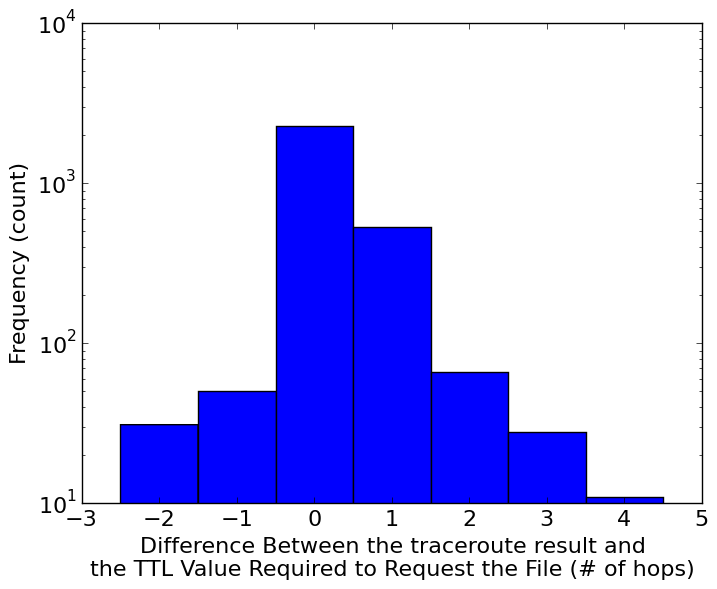
\includegraphics[width=\columnwidth]{figures/modifiedhist}
	\caption{
		A histogram of the same data from \ref{fig_gcprobehist} adjusted for updated \texttt{tcptraceroute} results in cases where the original result was 30 (and probably erroneous due to a failed traceroute).
		The one case where \texttt{tcptraceroute} never succeeded is not included in this adjusted plot.
	}
	\label{fig_modifiedhist}
\end{figure}